\chapter{Data Collection and Results}

\label{Chapter7_dataCollectionResults} 

\begin{comment}
-------------------------------------------------
%								Chapter layout
7. Data Collection and Results
	a. Data Collection Approach
	b. User Feedback
	c. Analysis of Control Data
	d. Goals Revisited
-------------------------------------------------
\end{comment}

Data collection for this project happened in two main ways. One was via the clinicians, who represented the clients who would be using the software this project built on patients in John Radcliffe Hospital. The other way was through myself reaching out to students and other people around my college to ask them if they would like to participate in the data collection part of my MSc project. I will also show some of the user feedback I received. Then some analysis of the control data collect via the application will be discussed; after which the original goals of this project revisted. 

%------------------------------------------------
%	SECTION 1 Data Collection Approach
%------------------------------------------------
\section{Data Collection Approach}

Once I had finished the coding part of the project, I collected some control data by myself which was stored in the General folder in the application. I then decided to gather some more data from other students and members of my college. To do so, I prepared a small survey for my particpants (which is shown in Appendix \ref{Appendix_survey}) that asked them some simple questions such as their general age bracket, their gender. The survey also had a question that asked the participants whether they preferred the vertical orientation fix done on the UI model after two versions of the application was shown to them, one with the vertical adjustment and one without. Every single participant found the vertical adjustment to be helpful towards the use-case the application was designed for. Lastly there was a question that asked them for "Any other comments." where they could express their overall impression of the application. To make it easier for the particpants I allowed them to speak their comments aloud and with their permission I was able to record them on my phone. I will be sharing some of the user feedback I received in the next section. 

The total amount of data I was able to gather accounted for 10 participants. Six of them were found by me and four of the particpants' data was sent to me by the clinicians. Of the participants I interviewed, 50 percent of them chose to be identified with the "Middle Age" age bracket and 50 percent chose the "Young Adult" option. Unfortunately I do not have the ages for the data sent to me by the clinicians, but I would assume they probably fell in one of these age groups also. In terms of gender distribution, 3 of the participants were female, while the other 7 were male. 

In gathering this data, I was reminded of my Requirements Engineering course work. The final project in the module also had a component for which we had to go out into the enviroment of the technological artifact that we chose for our study and collect some data about its use. That final project was very good because it forced me to go out and collect data from people. I used the same skills I learned then to help me collect data about this project. As simple as it looks, I feel approaching relative strangers can be a bit difficult. It makes one feel embarassed to bother them when they might be busy. However as I learned from my Requirements Engineering project and this final MSc project, this process gets easier the more one practices. One thing that I feel helped me to feel less guilty about taking people's time in a very busy time of the year was that I bought chocolate candies as a token of gratitude for their time. These were given as the end of the data collection and subsequent discussion; every particpant enjoyed this little surprise. One of the biggest takeaways for me during the process was the confidence I gained. 

%------------------------------------------------
%	SECTION 2 User Feedback
%------------------------------------------------
\section{User Feedback}
In this section, I will showcase some of the feedback that users of the application gave. The responses gathered were all positive with some suggestions about what could be changed. For example one participant was very enthusiastic about the whole process and felt it was a bit like game. In his feedback, he gave suggestions as to how this application could be even more "gameified" to attract the users to practice it more. This was definitely a good suggestion and could be one of the directions taken for a future project in this area. Here are some actual quotes from participants testing the application:

"In the begining, it took a bit of training to get used to it. But, after a couple of minutes, I got quicker at it. By the time I got to my right hand, I felt as if I was becoming more adept. And while it took a bit to master the configuration to mirror what was on the screen, I realized that it wasn't completely neccessary to do that. There are the algorthims there that recognize when I have got the correct hand gestures. So, I felt more relaxed when I knew that. But.. apart from that, it certainly got the coordinations of my hand and arm muscles going." --Andrew

"It was fun to do. It is a good exercise. Excellent intentions... I had to splay the hand immediately, and then configuring the hand became much easier. I kept the hand as much as I could in a horizontal attitude, but also there was a tendency to forget about where the hand was going. And actually the hand tended to descend more to the sensor, which you have mentioned that I have got to keep a certain distance. That was a little issue, as long as I remember that its fine." --Timothy

"Do you think it would be useful to have an element of a game-like scenario? To be quite honest, its fun to do. As in, you know, you want to do your best out there. I want to mimic it much as possible." --Zhang

"I thought it was quite easy to use. I like that it didn't seem to crash. It gave quite a dynamic and live view of your hand. It didnt seem to stress and freeze up. Once you have a trial, then yea, its easier. Once you realize that you put your hand in certain positions, you learn a bit more about how it works." --Amber

"I think some training is important. The feedback on the screen is a little bit confusing sometimes because sometimes it doesn't mimic exactly what you are doing. Sometimes there is cross-feedback going back and forth; I am trying to adapt to what I see on the screen but the screen is supposed to adapt to me. I think the rotation feature of the application is helpful, as is the vertical adjustment of the user's hand" --Paul

Above were some comments from users testing the application. The participants quickly became adept at understanding how to use the application. For example one of the things that one has to do from time to time when using the Leap Motion sensor is open the hand fully with the palm facing downwards. This is to recalibrate the device if it starts not behaving correctly because of occulsion, which is when some of the fingers below cover the fingers above and the device is unable to collect good data about the hand. After telling participants about this, most of them were able to resolve issues of the computer screen model not replicating their real hand's gesture fully. The particpants would quickly reopen their hand and try again and often the issue they would be having would be resolved. Sometimes particpants would forget to keep their hand in an area above the device. They would unconsiously move their hand too forward or too much to the side. Of course, these kind of problems would quickly resolve themselves through just a little bit of more training and practice. 


%------------------------------------------------
%	SECTION 3 Analysis of Control Data
%------------------------------------------------
\section{Analysis of Control Data }
In this section, I will briefly discuss the scoring results of the data collected in testing the useability of this application and the gesture comparison methods it implements. In the Figure \ref{fig:leftAvgs} we can see the average scores for the 10 left handed gestures. The first bar shows the score as determined by the Angle based scoring algorithm. 
\begin{figure}[H]
\centering
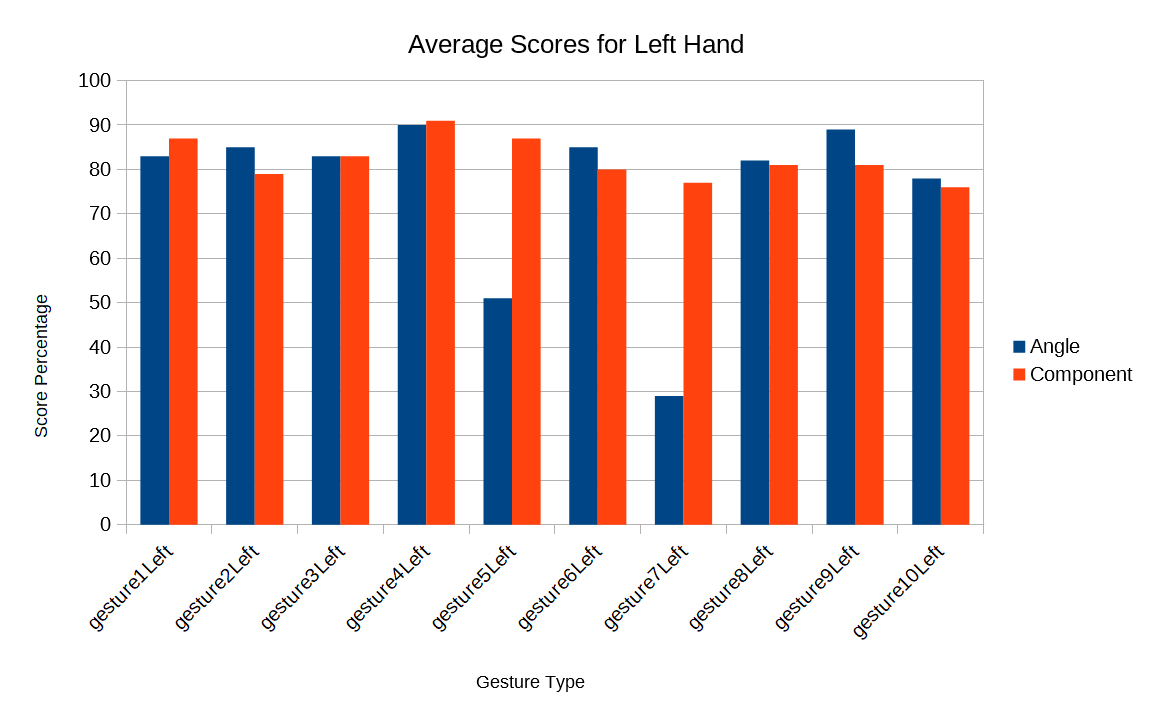
\includegraphics[scale=0.75]{Figures/7_avgLeft.JPG}
\caption[Averages for Left Hand Gestures]{The average scores for the 10 left hand gestures based upon the Angle and Component comparison functions.}
\label{fig:leftAvgs}
\end{figure}
The results were very good for both algorthims for most of the gestures considered. However, there is a noticable dip in the Angle based blue bar for gesture7Left. This gesture is the one where only the pinky is extended and all of the other fingers are curled in; a picture of this gesture is shown in Figure \ref{fig:gesture7Leftagain}.
\begin{figure}[H]
\centering
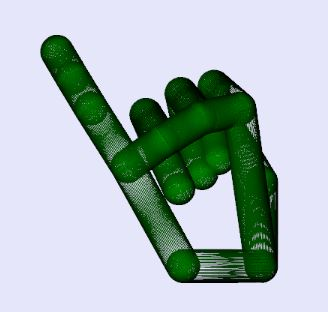
\includegraphics[scale=0.75]{Figures/gesture7Left.JPG}
\caption[Gesture7Left]{Gesture7Left, which is all of the fingers curled expect for the pinky.}
\label{fig:gesture7Leftagain}
\end{figure}
The reason why the Angle based score was so low for this figure was because this Angle based comparison function returned a zero value for five of the users tested. This zero value is automatically returned by the algorithm if the user hand and target hand passed into it are of opposite types; i.e. right hand compared with left hand will always return zero. Therefore, it is plausible the that for this gesture, the Leap Motion sensor confused some user hands showing gesture7Left to be showing a right hand with the thumb extended. This would have caused the many zeros and thus the low score for gesture7Left. Another gesture that scored a little bit poorly for the Angle based algorithm was gesture5Left. For this gesture, there were not any zeros recorded but it did receive pretty low scores for five users. Since the Angle based algorithm depends on the target hand for the comparison, I feel these low scores some users recieved might have been due to the fact that their gesture wasn't matching the target hand closely. The target hand used for this gesture could itself have been a little bit better also. It's a little bit sub-par. This deficency could explain the low score observed for gesture5Left. Other than these two gestures, all other averages are very good. And even for these two bad cases the low averages were caused by a few bad apples; the scores for these two problem cases were not low all around. 

Below is a chart, Figure \ref{fig:rightAvgs}, that shows the average scores for the 10 right handed gestures.
\begin{figure}[H]
\centering
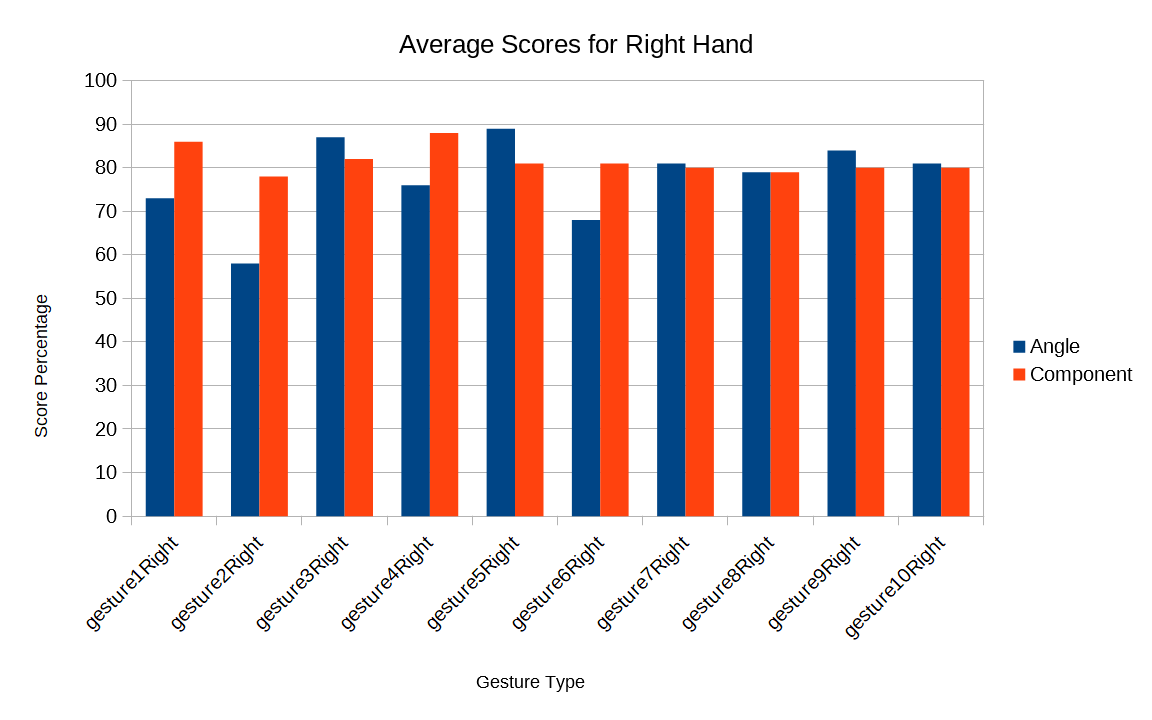
\includegraphics[scale=0.75]{Figures/7_avgRight.JPG}
\caption[Averages for Right Hand Gestures]{The average scores for the 10 right hand gestures based upon the Angle and Component comparison functions.}
\label{fig:rightAvgs}
\end{figure}
The chart shows that most of the right hand gesture data collected scored relatively high for all hands. The only is gesture2Right's Angle based score which is below 60 percent. However, that is again caused by just two users who scored very low for that gesture. A file containing all of the scoring data is shown in Appendix  Appendix \ref{Appendix_dataAvgs}. 

%------------------------------------------------
%	SECTION 4 Goals Revisited
%------------------------------------------------
\section{Goals Revisited}
Throughout the course of this entire project, I met with the clinicians, Dr Samrah Ahmed, Dr Christopher Butler, and Nikolas Drummond, several times to discuss the application as it was being designed and built. The features they requested were implemented in this software. In the final visit to the hospital, the complete version of the application was delivered for the clinicians for testing and collecting some control data. They feedback received from them was very positive. All of their major requested features were implemented satisfactorily. These goals include creating an easy to use application interface that allows the clinicians to collect data from patients. This data can be analyzed via two algorithms which grade the patients attempted hand gestures. The application provides the clinicians a scene to view the data that they collect and make appropriate modifications as they need to. One of the requests from the clinicians that surfaced during one of the meetings was the need to have a way for the patients to observe the hand gesture from variaty of angles. This goal was also satisfactorily completed by providing a button that rotates the 3D camera around the user and target hand. The application allows the clinicians to save/load the data to/from an external CSV file. In addition the application allows for the user to perform the gestures in a variaty of hand orientations and all the while shows the user a set vertical position on the screen. An additional benefit of this is that no additional rig or frame is required in order to collect good data from patients. Thus, the main UI and usabiltiy goals of this project were met.















